\documentclass{article}
\usepackage{tikz,geometry,marvosym}
\usetikzlibrary{arrows,positioning,calc,fit}
\usepackage[T1]{fontenc}
\usepackage[utf8]{inputenc}
\pagestyle{empty}
\geometry{
paperwidth=12.3cm,
paperheight = 4.8cm,
left=0pt,
right=0pt,
top=2pt,
bottom=0pt
}
\tikzset{
interagit/.style={stealth-stealth},
master/.style={open diamond-}
}
\pgfdeclarelayer{background}
\pgfsetlayers{background,main}
\begin{document}
\centering
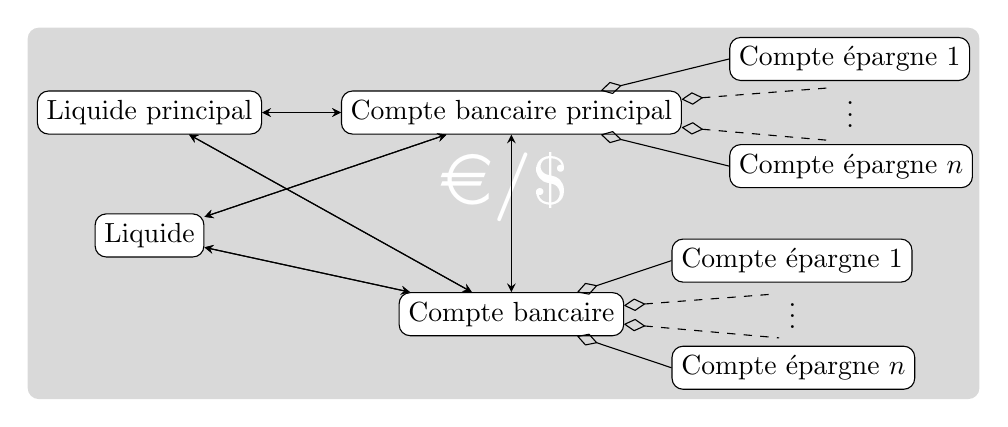
\begin{tikzpicture}[every node/.append style={align=left,draw,rounded corners,fill=white}]
%%% banque princ & epargne
\node (bank0) at (0,0) {Compte bancaire principal};
\node[above right=4mm and 6mm] (epa01)  at (bank0.east) {Compte épargne 1};
\node[below right=4mm and 6mm] (epa02)  at (bank0.east) {Compte épargne $n$};
\node[draw=none,fill=none] at ( $(epa01.south)!0.4!(epa02.north)$ ) {$\vdots$};
\foreach \i in {10,-10}
  \draw[master,dashed] (bank0) -- ( $(bank0)!0.9!\i:(epa01.south)!0.5!(epa02.north)$);
\foreach \i in {1,2}
  \draw[master] (bank0) -- (epa0\i.west);
%%%%% liquides
\node[left=1cm]  (liq0) at (bank0.west) {Liquide principal};
\node[below=1cm] (liq1) at (liq0.south) {Liquide};
%%%
\node[below=2cm] (bank1) at (bank0.south) {Compte bancaire};
\node[above right=4mm and 6mm] (epa11)  at (bank1.east) {Compte épargne 1};
\node[below right=4mm and 6mm] (epa12)  at (bank1.east) {Compte épargne $n$};
\node[draw=none,fill=none] at ( $(epa11.south)!0.4!(epa12.north)$ ) {$\vdots$};
\foreach \i in {10,-10}
  \draw[master,dashed] (bank1) -- ( $(bank1)!0.9!\i:(epa11.south)!0.5!(epa12.north)$);
\foreach \i in {1,2}
  \draw[master] (bank1) -- (epa1\i.west);
%%liquide & bank interact
\foreach \il in {0,1}
{
 \foreach \ib in {0,1}
 {
  \draw[interagit] (liq\il) -- (bank\ib);
  \draw[interagit] (liq\il) -- (bank\ib);
 }
}
\draw[interagit] (bank0) -- (bank1);
\begin{pgfonlayer}{background}
\node[draw=none,fill=gray!30, fit = (epa01) (liq0) (epa12),text=white,font=\bf\Huge] {\EUR/\$};
\end{pgfonlayer}
\end{tikzpicture}
\end{document}
